
\chapter{Fundamentos}\label{chap:fundamentos}


\section{Fundamentos de la tomografía computarizada}\label{sec:fundamentos_TC}

La tomografía computarizada es una técnica de imagen médica basada en rayos X que permite obtener representaciones transversales del interior del cuerpo humano. A diferencia de la radiografía convencional, que proyecta un volumen tridimensional sobre una imagen bidimensional y provoca la superposición de estructuras anatómicas, la TC reconstruye cortes internos del paciente a partir de múltiples medidas adquiridas desde diferentes ángulos \cite{buzug2011computed}. Esta capacidad de representar secciones anatómicas sin solapamiento convierte a la TC en una herramienta especialmente útil para el estudio de estructuras internas complejas, como el tórax y el parénquima pulmonar.

Desde su introducción clínica a comienzos de la década de 1970, la TC ha evolucionado desde sistemas inicialmente orientados al estudio craneal hasta equipos capaces de adquirir volúmenes completos de distintas regiones anatómicas \cite{calzado2010tomografia,schulz2021ct}. Esta evolución ha estado ligada tanto a mejoras en la adquisición de datos, como la incorporación de escáneres helicoidales y multidetectores, como al desarrollo de algoritmos de reconstrucción más eficientes. En el contexto de este trabajo, esta evolución resulta especialmente relevante, ya que los estudios disponibles no se analizan como imágenes aisladas, sino como volúmenes tridimensionales formados por múltiples cortes axiales.

El principio físico de la TC se basa en la atenuación diferencial de los rayos X al atravesar los tejidos. Cuando el haz de rayos X atraviesa el cuerpo, cada tejido atenúa la radiación en función de su composición y densidad. Los detectores registran la intensidad del haz tras atravesar al paciente y, a partir de las proyecciones obtenidas en diferentes orientaciones, se reconstruye una imagen que representa la distribución espacial de los coeficientes de atenuación. Tradicionalmente, una de las técnicas fundamentales de reconstrucción ha sido la retroproyección filtrada o \textit{filtered back projection} (FBP), que permite obtener cortes tomográficos a partir de las proyecciones adquiridas \cite{schofield2020image}.

El resultado de este proceso es una imagen formada por píxeles en el plano bidimensional. Cuando se consideran múltiples cortes consecutivos, estos píxeles se extienden a vóxeles, que representan unidades de volumen dentro del espacio tridimensional. Cada vóxel contiene información sobre la atenuación del tejido correspondiente, por lo que el conjunto de cortes de TC puede interpretarse como un volumen anatómico. Esta representación volumétrica es la que permite aplicar posteriormente técnicas de análisis tridimensional, extracción de características radiómicas o modelos de aprendizaje profundo 3D.

Para estandarizar los valores de atenuación y facilitar su interpretación clínica, las intensidades de la TC se expresan en unidades Hounsfield (HU), tomando como referencias el agua y el aire \cite{calzado2010tomografia}. La conversión se define como:

\[
HU_{mat} = \frac{\mu_{mat} - \mu_{agua}}{\mu_{agua}} \times 1000
\]

donde $\mu_{mat}$ representa el coeficiente de atenuación lineal del tejido o material considerado, y $\mu_{agua}$ el coeficiente de atenuación correspondiente al agua. Esta escala permite asociar distintos rangos de intensidad a diferentes tipos de tejido: el aire se sitúa aproximadamente en $-1000$ HU, el agua en 0 HU, el tejido adiposo suele encontrarse entre $-100$ y $-80$ HU, el parénquima pulmonar presenta valores negativos debido a su contenido aéreo, y las estructuras óseas pueden alcanzar valores superiores a $+1000$ HU.

Sin embargo, el rango completo de intensidades HU es demasiado amplio para visualizar todos los tejidos con el mismo nivel de contraste. Por este motivo, en la práctica clínica se emplean ventanas de visualización, definidas mediante dos parámetros: el \textit{Window Level} (WL), que establece el valor central de la ventana, y el \textit{Window Width} (WW), que determina la amplitud del intervalo representado. La selección de diferentes ventanas permite resaltar estructuras concretas, como el parénquima pulmonar, el mediastino o el hueso. Este concepto resulta especialmente importante en este trabajo, ya que las ventanas HU se utilizan posteriormente durante el preprocesamiento de los volúmenes para resaltar información anatómica relevante.

Una vez reconstruido el volumen de TC, este puede visualizarse en diferentes planos anatómicos. El plano axial corresponde a los cortes transversales adquiridos habitualmente durante el estudio; el plano sagital permite observar el cuerpo desde una perspectiva lateral; y el plano coronal proporciona una vista frontal. La posibilidad de reformatear el volumen en estos planos, conocida como reformateo multiplanar o \textit{Multiplanar Reformation} (MPR), es una de las ventajas principales de la TC volumétrica, ya que facilita la interpretación anatómica desde distintas orientaciones.

\begin{figure}[!htbp]
    \centering
    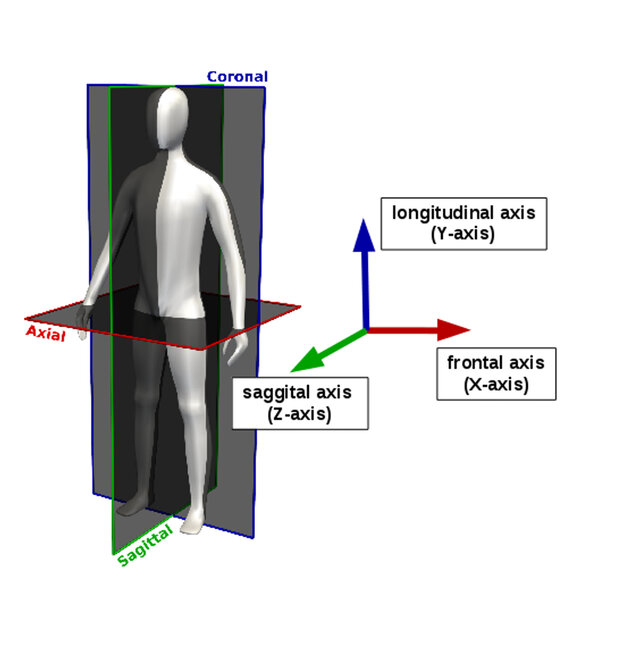
\includegraphics[width=0.7\textwidth]{imagenes/fundamentos/ejes_ct.jpg}
    \caption{Visualización de los planos anatómicos estándar en tomografía computarizada: axial, sagital y coronal. En el sistema de coordenadas mostrado, el eje X corresponde al eje frontal o izquierda-derecha, el eje Y al eje longitudinal o cráneo-caudal, y el eje Z al eje sagital o antero-posterior. Fuente: \cite{heim2018large}.}
    \label{fig:ct_ejes_anatomicos}
\end{figure}

Además del reformateo multiplanar, los volúmenes de TC pueden representarse mediante técnicas de visualización tridimensional, como el renderizado de volumen o el renderizado de superficie. No obstante, en el contexto de este trabajo, el interés principal de la TC reside en su naturaleza volumétrica y cuantitativa, ya que proporciona información espacial e intensidades HU que pueden ser utilizadas tanto en análisis radiómico como en modelos de inteligencia artificial aplicados a imagen médica.




% \section{Fundamentos de aprendizaje automático supervisado en medicina??}
%     \subsection{Clasificación binaria y clasificación multietiqueta}
%     \subsection{Desbalanceo de clases}
%     \subsection{Validación cruzada y separación entrenamiento-validación-test}
%     \subsection{Métricas de evaluación en problemas clínicos}




\section{Fundamentos matemáticos de la radiómica}

En esta sección se explican los fundamentos de la radiómica necesarios para la parte práctica del capítulo~\ref{chap:radiomica}.

La radiómica es una metodología de análisis de imagen médica orientada a transformar imágenes o volúmenes médicos en un conjunto de características cuantitativas. Estas características describen propiedades de intensidad, forma, textura y distribución espacial de los tejidos, y pueden utilizarse posteriormente como variables de entrada en modelos estadísticos o de aprendizaje automático. En el contexto de la medicina de precisión, la radiómica parte de la hipótesis de que determinadas propiedades biológicas o clínicas de una lesión pueden reflejarse de forma indirecta en la imagen médica, permitiendo extraer información adicional a la observación visual convencional \cite{demathematical}. Este proceso se resume de forma esquemática en la Figura~\ref{fig:radiomica-cancer}.

\begin{figure}[!htbp]
    \centering
    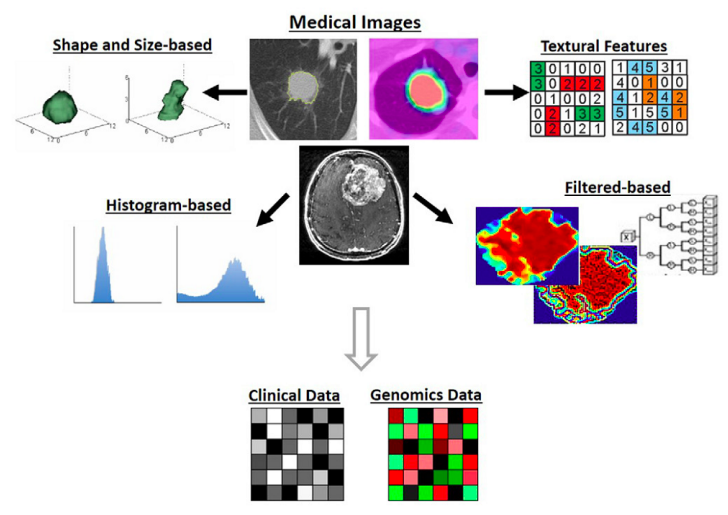
\includegraphics[width=0.9\textwidth]{imagenes/fundamentos/radiomica_cancer.png}
    \caption{Principio general de la radiómica y extracción de características cuantitativas a partir de imágenes médicas. A partir de la imagen original pueden obtenerse características de forma, intensidad, textura y filtrado, que posteriormente pueden combinarse con información clínica o genómica. Fuente: \cite{demathematical}.}
    \label{fig:radiomica-cancer}
\end{figure}


A diferencia de la interpretación radiológica clásica, basada principalmente en la inspección visual de las imágenes, la radiómica busca obtener medidas objetivas y reproducibles. Para ello, es necesario definir previamente una región o volumen de interés sobre el que calcular las características. En imágenes bidimensionales se habla de región de interés o ROI (\textit{Region of Interest}), mientras que en estudios tridimensionales, como los volúmenes de tomografía computarizada, se utiliza el concepto de volumen de interés o VOI (\textit{Volume of Interest}). El VOI queda formado por el conjunto de vóxeles pertenecientes a la estructura anatómica o lesión que se desea estudiar. Esta explicación se basa en \textit{Image biomarker standardisation initiative (IBSI)}\footnote{\url{https://theibsi.github.io/}} y la documentación de \textit{PyRadiomics}\footnote{\url{https://pyradiomics.readthedocs.io/en/latest/}}. 

Siguiendo la formulación propuesta por la \textit{Image Biomarker Standardisation Initiative} (IBSI), una imagen médica tridimensional puede representarse como una función discreta definida sobre una rejilla de vóxeles \cite{zwanenburg2020image}. De forma general, cada vóxel queda identificado por sus coordenadas espaciales $(x,y,z)$ y por un valor de intensidad asociado:

\[
I(x,y,z), \quad x=1,\ldots,X,\quad y=1,\ldots,Y,\quad z=1,\ldots,Z
\]

donde $X$, $Y$ y $Z$ representan las dimensiones del volumen.

Por tanto, la extracción radiómica consiste en aplicar funciones matemáticas sobre los vóxeles contenidos en dicho VOI para obtener un conjunto de descriptores cuantitativos. El resultado puede expresarse como un vector de características:

\[
\mathbf{f} = (f_1, f_2, \ldots, f_n)
\]

donde cada componente $f_i$ representa una medida concreta de la imagen, como una propiedad de forma, una estadística de intensidad o una medida de textura. 


Dentro de las familias de características definidas por IBSI se encuentran las características morfológicas o de forma, que describen la geometría del VOI y no dependen directamente de los valores de intensidad de la imagen \cite{zwanenburg2020image}. Entre ellas se incluyen medidas como el volumen, la superficie o la esfericidad. De forma simplificada, el volumen físico de una región segmentada puede calcularse a partir del número de vóxeles contenidos en el VOI y del tamaño físico de cada vóxel:

\[
V = N_v \cdot v_x \cdot v_y \cdot v_z
\]

donde $N_v$ es el número de vóxeles de la región segmentada, y $v_x$, $v_y$ y $v_z$ representan las dimensiones físicas del vóxel en cada dirección espacial. Esta magnitud permite cuantificar el tamaño de la región analizada y constituye una de las medidas básicas de forma en radiómica.


Las características de primer orden describen la distribución de intensidades dentro del VOI sin considerar de forma explícita la relación espacial entre vóxeles. Siguiendo la formulación de IBSI, estas características se calculan a partir de los valores de intensidad contenidos en la región segmentada, normalmente resumidos mediante un histograma \cite{zwanenburg2020image}. Si $h(i)$ representa el número de vóxeles con intensidad o nivel discretizado $i$, la probabilidad asociada a dicho nivel puede expresarse como:

\[
p(i) = \frac{h(i)}{N_v}
\]

donde $N_v$ es el número total de vóxeles del VOI. A partir de esta distribución se obtienen medidas estadísticas que resumen la intensidad de la región. Por ejemplo, la media representa el valor promedio de intensidad:

\[
\mu = \sum_i i \, p(i)
\]

mientras que la varianza mide la dispersión de las intensidades respecto a dicha media:

\[
\sigma^2 = \sum_i (i-\mu)^2 p(i)
\]

Otra medida habitual es la entropía, que cuantifica el grado de heterogeneidad o desorden de la distribución de intensidades:

\[
H = -\sum_i p(i)\log_2 p(i)
\]

De este modo, regiones con intensidades muy similares tienden a presentar valores bajos de entropía, mientras que regiones con mayor variabilidad interna presentan valores más elevados. Estas características permiten resumir la información global de intensidad del VOI, pero no describen cómo se organizan espacialmente los vóxeles dentro de la región.

Para capturar dicha organización espacial se emplean características de textura. Estas medidas analizan no solo qué intensidades aparecen en el VOI, sino también cómo se distribuyen y relacionan entre sí. De acuerdo con la clasificación estandarizada por IBSI, las características texturales se calculan a partir de matrices que codifican distintos tipos de relaciones espaciales entre niveles de gris \cite{zwanenburg2020image}. Entre las familias más utilizadas se encuentran:

\begin{itemize} 
    \item \textbf{Matriz de coocurrencia de niveles de gris (GLCM, \textit{Gray Level Co-occurrence Matrix})}: introducida por Haralick et al. \cite{haralick2007textural}, describe la frecuencia con la que aparecen pares de niveles de gris en una relación espacial determinada, definida por una distancia y una dirección. A partir de esta matriz se pueden calcular características como el contraste, la correlación, la energía o la homogeneidad. 
    \item \textbf{Matriz de dependencia de niveles de gris (GLDM, \textit{Gray Level Dependence Matrix})}: propuesta por Amadasun y King \cite{amadasun1989textural}, permite describir dependencias entre un vóxel y sus vecinos. Para cada nivel de gris, considera grupos de vóxeles adyacentes cuya intensidad es similar dentro de un umbral determinado, proporcionando información sobre la dependencia local de intensidades. 
    \item \textbf{Matriz de longitud de recorridos de niveles de gris (GLRLM, \textit{Gray Level Run Length Matrix})}: introducida por Galloway \cite{galloway1974texture}, caracteriza la longitud de secuencias consecutivas de vóxeles con el mismo nivel de gris en una dirección concreta. Esta matriz permite describir patrones relacionados con la uniformidad, la granularidad y el tamaño de estructuras texturales. 
    \item \textbf{Matriz de zonas de tamaño de niveles de gris (GLSZM, \textit{Gray Level Size Zone Matrix})}: propuesta por Thibault et al. \cite{thibault2013advanced}, cuantifica el tamaño de zonas conectadas con el mismo nivel de gris, independientemente de la dirección. A diferencia de la GLRLM, no depende de una orientación específica, por lo que permite describir la distribución de regiones homogéneas de distinto tamaño. 
\end{itemize}

Estas matrices permiten extraer características que reflejan diferentes aspectos de la textura, como la homogeneidad, el contraste, la complejidad o la presencia de patrones repetitivos. Por ejemplo, una región con intensidades similares entre vóxeles vecinos tenderá a presentar mayor homogeneidad, mientras que una región con cambios bruscos de intensidad mostrará mayor contraste y heterogeneidad.



% \section{Fundamentos de aprendizaje automático clásico para datos clínicos y radiómicos??}
%     \subsection{Regresión logística y modelos lineales}
%     \subsection{Árboles de decisión y Random Forest}
%     \subsection{Gradient boosting: XGBoost y LightGBM}
%     \subsection{KNN, SVM y modelos basados en distancia}
%     \subsection{Interpretabilidad básica de modelos tabulares}

% \section{Fundamentos de deep learning para imagen médica volumétrica??}
%     \subsection{Redes convolucionales 2D, 2.5D y 3D}
%     \subsection{Aprendizaje de representaciones en volúmenes médicos}
%     \subsection{Transfer learning y preentrenamiento}
%     \subsection{Fusión de datos imagen-tabular}
%     \subsection{Principales limitaciones en cohortes pequeñas}

\section{Fundamentos de Positive-Unlabeled Learning}\label{sec:fundamentos_pu}
    % \subsection{Planteamiento del problema positivo-sin-etiquetas}
    % \subsection{Diferencia entre aprendizaje supervisado, semisupervisado y PU Learning}
    % \subsection{Supuestos SCAR, SAR y sesgo de selección}
    % \subsection{Estimación del prior de clase}
    % \subsection{Estrategias de modelado PU}
    % \subsection{Evaluación de modelos PU en contexto clínico}

    El aprendizaje positivo-sin-etiquetar, conocido como \textit{Positive-Unlabeled Learning}, aborda problemas de clasificación binaria en los que solo se dispone de positivos identificados y de un conjunto no etiquetado. A diferencia del aprendizaje supervisado convencional, no se conoce un conjunto fiable de ejemplos negativos porque las observaciones no etiquetadas pueden contener tanto negativos reales como positivos que no han sido identificados. Tampoco se trata de un problema semisupervisado estándar, ya que en este último suelen existir ejemplos etiquetados de todas las clases, mientras que en PU learning solo una de ellas está explícitamente representada \cite{Elkan2008,Bekker2020}.

    Sea \(y\in\{0,1\}\) la clase real de una observación y \(s\in\{0,1\}\) el indicador de que esta ha sido etiquetada como positiva. La formulación PU supone que una observación etiquetada es realmente positiva,

    \[
    P(y=1\mid s=1)=1,
    \]

    mientras que para las observaciones con \(s=0\) la clase real permanece desconocida. Por tanto, el conjunto de entrenamiento puede expresarse como

    \[
    D = P \cup U,
    \]

    donde \(P=\{(\mathbf{x}_i,s_i):s_i=1\}\) contiene los positivos observados y \(U=\{(\mathbf{x}_i,s_i):s_i=0\}\) representa el conjunto no etiquetado.

    Uno de los supuestos más habituales es el denominado \textit{Selected Completely At Random} (SCAR). Bajo este supuesto, todos los positivos reales tienen la misma probabilidad \(c\) de ser etiquetados, con independencia de sus características:

    \[
    P(s=1\mid y=1,\mathbf{x})=c,
    \qquad
    P(s=1\mid y=0,\mathbf{x})=0.
    \]

    El valor \(c\) representa, por tanto, la probabilidad de que un ejemplo realmente positivo aparezca etiquetado como tal. Si un clasificador entrenado para distinguir positivos observados de ejemplos no etiquetados estima

    \[
    g(\mathbf{x})=P(s=1\mid\mathbf{x}),
    \]

    la probabilidad de pertenecer a la clase positiva puede corregirse como

    \[
    P(y=1\mid\mathbf{x})
    =
    \min\left(\frac{g(\mathbf{x})}{c},1\right).
    \]

    Esta es la base del método de Elkan y Noto \cite{Elkan2008}. En la práctica, \(c\) puede estimarse a partir de las puntuaciones obtenidas para positivos que no hayan sido utilizados para ajustar el modelo, por ejemplo mediante predicciones fuera de muestra. Esta separación resulta importante para evitar estimaciones excesivamente optimistas.

    Las estrategias PU pueden agruparse en varios enfoques. Una aproximación sencilla consiste en tratar provisionalmente todo el conjunto no etiquetado como negativo, aunque esta decisión introduce ruido cuando contiene positivos ocultos. Otras alternativas buscan identificar negativos suficientemente fiables, corrigen las probabilidades mediante la estimación de \(c\), entrenan múltiples clasificadores sobre diferentes muestras del conjunto no etiquetado o reformulan directamente el riesgo de clasificación. Dentro de este último grupo, los estimadores de riesgo no negativo limitan el riesgo empírico para reducir el sobreajuste que puede aparecer con modelos flexibles \cite{Kiryo2017}.

El método \textit{non-negative Positive-Unlabeled Learning} (nnPU) pertenece a esta última familia y permite entrenar modelos flexibles, como las redes neuronales, directamente a partir de positivos observados y casos no etiquetados. El estimador PU no sesgado puede producir durante el entrenamiento una contribución negativa del riesgo asociado a la clase negativa, favoreciendo el sobreajuste a los positivos observados. nnPU evita este comportamiento limitando dicha contribución para que no sea negativa. Su aplicación requiere estimar previamente el prior de la clase positiva, que determina el peso relativo de los términos del riesgo \cite{Kiryo2017}.

    La validez de estos métodos depende del mecanismo mediante el cual se han observado las etiquetas. Si los casos positivos más graves o más evidentes tienen mayor probabilidad de ser registrados, el supuesto SCAR puede incumplirse y aparecer un escenario de selección dependiente de las características. Por ello, PU learning no demuestra por sí mismo que existan positivos ocultos ni permite recuperar automáticamente las etiquetas reales. En este trabajo se emplea como un análisis de sensibilidad ante una posible incertidumbre en el registro de las complicaciones, comparando sus resultados con los obtenidos mediante aprendizaje supervisado convencional.



\section{Fundamentos de Subgroup Discovery} \label{sec:fundamentos_subgroup_discovery}

El descubrimiento de subgrupos o \textit{subgroup discovery} es una tarea de minería de datos descriptiva orientada a identificar subconjuntos de una población que presentan un comportamiento inusual respecto de una propiedad de interés. Sus antecedentes se encuentran en los primeros sistemas de descubrimiento de patrones y su formulación se ha consolidado posteriormente como un área situada entre la inducción predictiva y la descriptiva \cite{Herrera2011,Atzmueller2015}. El objetivo no consiste en construir un modelo global que asigne una clase a todos los individuos, sino en obtener descripciones locales, comprensibles y potencialmente útiles de determinados segmentos de la población.

Esta orientación permite diferenciar el descubrimiento de subgrupos de otras tareas de aprendizaje. En clasificación supervisada se busca principalmente maximizar la capacidad predictiva sobre observaciones no vistas, mientras que en \textit{subgroup discovery} se pretende caracterizar regiones concretas del espacio de datos que presentan una distribución particular de la variable objetivo. Frente al agrupamiento no supervisado, la búsqueda está guiada por una propiedad de interés previamente definida y los subgrupos resultantes pueden solaparse, por lo que no constituyen necesariamente una partición de la población. También se relaciona con la minería de conjuntos de contraste y de patrones emergentes, enfoques que han sido agrupados bajo el concepto más general de descubrimiento supervisado de reglas descriptivas \cite{KraljNovak2009}. Esta naturaleza local y descriptiva explica su interés en dominios clínicos, donde puede ser más informativo reconocer perfiles concretos de pacientes que resumir toda la población mediante un único modelo \cite{Gamberger2002,Esnault2020}.

\subsection{Representación de los subgrupos}

Sea un conjunto de datos $D=\{(\mathbf{x}_i,y_i)\}_{i=1}^{N}$, donde $\mathbf{x}_i$ representa las variables descriptivas del individuo $i$ e $y_i$ la propiedad objetivo. Un subgrupo se define mediante una descripción $C$, formada habitualmente por una conjunción de condiciones interpretables sobre las variables de entrada. El conjunto de individuos cubiertos por dicha descripción es

\[
S_C = \{i \in \{1,\ldots,N\} : C(\mathbf{x}_i)=\mathrm{verdadero}\}.
\]

Cuando el objetivo es binario, el patrón puede expresarse mediante una regla

\[
R: C \rightarrow y=1.
\]

El antecedente $C$ puede incluir selectores categóricos, como $x_j=v$, y condiciones sobre variables numéricas, como $x_j\leq t$ o $a<x_j\leq b$. La elección del lenguaje de descripción determina qué subgrupos pueden descubrirse y condiciona tanto la interpretabilidad como la complejidad del espacio de búsqueda. En particular, una discretización previa demasiado rígida de las variables continuas puede excluir intervalos informativos, mientras que permitir demasiados umbrales incrementa de forma considerable el número de reglas candidatas \cite{Meeng2021}.

Las reglas de subgrupos son parciales: no tienen que cubrir toda la población y distintas reglas pueden incluir a los mismos individuos. Además, su consecuente se fija de acuerdo con la propiedad que se desea estudiar, a diferencia de las reglas de asociación generales, en las que tanto el antecedente como el consecuente forman parte del proceso de búsqueda. Esta formulación facilita que cada patrón pueda leerse como una descripción explícita de las condiciones bajo las cuales la propiedad objetivo aparece con una distribución distinta de la observada globalmente \cite{Herrera2011,Atzmueller2015}.

\subsection{Medidas de calidad}

La utilidad de una regla no depende únicamente de su precisión, sino también del número de observaciones que describe y de la diferencia que introduce respecto de la distribución global. Sea $n(C)=|S_C|$ el número de individuos cubiertos por el antecedente, $n(y)$ el número total de individuos con $y=1$ y $n(C,y)$ el número de individuos cubiertos que presentan el objetivo. A partir de estos recuentos se definen varias medidas básicas:

\[
\operatorname{Cobertura}(C)=\frac{n(C)}{N},
\qquad
\operatorname{Soporte}(C\rightarrow y)=\frac{n(C,y)}{N},
\]

\[
\operatorname{Confianza}(C\rightarrow y)=\frac{n(C,y)}{n(C)},
\qquad
\operatorname{Sensibilidad}(C\rightarrow y)=\frac{n(C,y)}{n(y)}.
\]

La cobertura cuantifica la proporción de la población descrita por la regla, mientras que el soporte incorpora simultáneamente el antecedente y el objetivo. La confianza representa la prevalencia del objetivo dentro del subgrupo y la sensibilidad indica qué proporción de todos los individuos positivos queda cubierta. Ninguna de estas medidas resulta suficiente de forma aislada: una regla puede alcanzar una confianza elevada apoyándose en muy pocos individuos, o cubrir una parte amplia de la población sin aportar una desviación relevante respecto de la prevalencia basal.

Una medida especialmente utilizada es la precisión relativa ponderada, conocida como \textit{Weighted Relative Accuracy} (WRAcc) o \textit{unusualness}. Su expresión es

\[
\operatorname{WRAcc}(C\rightarrow y)
=
\frac{n(C)}{N}
\left(
\frac{n(C,y)}{n(C)}-\frac{n(y)}{N}
\right).
\]

Esta medida pondera la diferencia entre la prevalencia del objetivo dentro del subgrupo y su prevalencia global mediante la cobertura del antecedente. Un valor positivo indica que el objetivo está enriquecido dentro del subgrupo; un valor próximo a cero refleja que su frecuencia es similar a la de la población; y un valor negativo indica una menor presencia del objetivo. Otra medida habitual es el \textit{lift}, definido como

\[
\operatorname{Lift}(C\rightarrow y)
=
\frac{n(C,y)/n(C)}{n(y)/N},
\]

que expresa cuántas veces es mayor o menor la prevalencia local respecto de la global. Sin embargo, el \textit{lift} puede favorecer reglas con coberturas muy reducidas, por lo que debe interpretarse junto con recuentos absolutos, cobertura y soporte.

La calidad de un subgrupo también puede incorporar su simplicidad, novedad y significación. Las descripciones cortas suelen ser más comprensibles, mientras que conjuntos extensos de reglas muy similares dificultan la interpretación. Asimismo, una puntuación elevada de WRAcc, confianza o \textit{lift} no equivale a evidencia estadística ajustada: al examinar muchas reglas aumenta la probabilidad de encontrar patrones aparentemente interesantes por azar \cite{Duivesteijn2011}. Por ello, las medidas descriptivas de calidad, la magnitud del efecto, la incertidumbre estadística y la estabilidad deben considerarse dimensiones diferentes y complementarias.

\subsection{Estrategias de búsqueda y control de redundancia}

El número de descripciones posibles crece de forma combinatoria con el número de variables, valores y condiciones permitidas. Los algoritmos de descubrimiento de subgrupos combinan, por tanto, un lenguaje de refinamiento, una función de calidad y una estrategia de búsqueda. Entre las aproximaciones habituales se encuentran la búsqueda exhaustiva con poda, la búsqueda en haz o \textit{beam search}, las adaptaciones de algoritmos de clasificación y reglas de asociación, y los métodos evolutivos \cite{Herrera2011,Atzmueller2015}. CN2-SD constituye un ejemplo clásico de adaptación de un algoritmo de inducción de reglas de clasificación a una finalidad descriptiva, modificando el esquema de cobertura y la heurística para favorecer subgrupos suficientemente amplios e inusuales \cite{Lavrac2004}.

La búsqueda exhaustiva permite obtener garantías respecto de la función de calidad cuando se dispone de cotas optimistas capaces de descartar ramas que no pueden mejorar los resultados actuales. No obstante, su coste puede resultar prohibitivo en espacios de alta dimensión. La búsqueda en haz mantiene únicamente un número limitado de candidatos prometedores en cada nivel y reduce el coste computacional, aunque puede descartar de forma prematura regiones relevantes del espacio. Los métodos evolutivos y otras heurísticas ofrecen alternativas flexibles para optimizar simultáneamente varios criterios, pero tampoco garantizan necesariamente la recuperación del óptimo global.

Seleccionar simplemente las $k$ reglas con mayor puntuación suele generar variantes casi equivalentes que cubren a los mismos individuos. El descubrimiento de conjuntos diversos de subgrupos aborda este problema considerando la calidad conjunta y el solapamiento entre patrones, en lugar de ordenar cada regla de manera independiente \cite{VanLeeuwen2012}. Más recientemente, los modelos basados en listas de subgrupos han propuesto organizar reglas ordenadas que describen regiones diferentes de los datos. El enfoque de Proença et al. utiliza el principio de longitud mínima de descripción o \textit{Minimum Description Length} (MDL) para equilibrar excepcionalidad y complejidad, penalizar la exploración de numerosas hipótesis y obtener conjuntos compactos y no redundantes para objetivos univariantes o multivariantes \cite{Proenca2022}. Estos avances amplían la formulación clásica, centrada en encontrar reglas individuales de alta calidad, hacia modelos descriptivos globalmente interpretables y con mayor control del sobreajuste.

\subsection{Robustez e interpretación clínica}

El descubrimiento de subgrupos es, por naturaleza, una tarea exploratoria. La evaluación de numerosas combinaciones de variables, umbrales y objetivos introduce un problema de comparaciones múltiples: incluso cuando no existe una asociación real, alguna regla puede alcanzar una puntuación elevada debido al azar. Duivesteijn y Knobbe muestran que la validación debe considerar el proceso completo de búsqueda y no únicamente las reglas finalmente seleccionadas, por ejemplo mediante distribuciones nulas obtenidas por permutación \cite{Duivesteijn2011}. En datos clínicos, propuestas como Q-Finder combinan requisitos de tamaño mínimo, magnitud del efecto, significación, corrección por multiplicidad, diversidad y evaluación en datos separados para favorecer subgrupos más creíbles \cite{Esnault2020}.

En cohortes pequeñas resulta especialmente importante informar de los recuentos absolutos, limitar la longitud de las reglas, exigir un soporte mínimo y analizar la estabilidad de los patrones frente a cambios en la muestra. La validación puede estudiar tanto la estabilidad sintáctica, referida a la repetición de las mismas condiciones, como la estabilidad extensional, basada en el solapamiento entre los individuos cubiertos por reglas obtenidas en distintos remuestreos. Una regla sencilla y estable puede resultar más útil que otra con una puntuación ligeramente superior pero sustentada por pocos casos o muy sensible a la partición de los datos. Cuando no existe una cohorte externa, los patrones deben presentarse como hipótesis exploratorias pendientes de replicación independiente.

Finalmente, los subgrupos describen asociaciones locales y no establecen relaciones causales. Su interpretación debe apoyarse en la plausibilidad clínica, en la disponibilidad temporal de las variables y en la ausencia de fuga de información. En este trabajo, el planteamiento multietiqueta permite estudiar cada tipo de complicación como una propiedad objetivo binaria sin imponer exclusividad entre las distintas complicaciones, mientras que la ausencia de complicaciones se mantiene como una etiqueta explícita. Las etiquetas objetivo y las variables registradas después del procedimiento no deben formar parte de los antecedentes de las reglas. De este modo, el descubrimiento de subgrupos se emplea para obtener perfiles clínicos interpretables y generar hipótesis sobre la heterogeneidad de las complicaciones, no como sustituto de la evaluación predictiva ni como evidencia clínica confirmatoria.


% \section{Fundamentos de explicabilidad en modelos de IA médica??}
%     \subsection{Explicabilidad global y local}
%     \subsection{SHAP en modelos tabulares y radiómicos}
%     \subsection{Grad-CAM en modelos convolucionales}
%     \subsection{Utilidad y límites de la explicabilidad en medicina}